\chapter{LS\_NRA求解器的启发式前瞻机制与高效实现}\label{chap:implementation}

本章节主要介绍了LS\_NRA的整体框架和算法细节。除了前面两章介绍的胞腔跳跃缓存机制和等式松弛机制,本文还为非线性问题操作的停滞设计了简单的前瞻机制。然后,本文详细讨论本工具的具体实现,包括预处理阶段、重启策略、线性方程的快速运算、变量可行域的计算以及参数设置。

\section{启发式移动和前瞻机制}
如前文所述,非线性算术理论的一个挑战就是并不总是存在单变量的关键移动来满足一个特定的约束。之前的做法更多依赖于沿着固定直线的参数方程替代\cite{LiXZ23},更一般的做法需要用到柱形代数分解或多项式优化等理论。特别地,在SMT-LIB测试样例中,一类来自于生物网络\cite{AkutsuHT08}的名为Sturm-MBO的样例覆盖了大量的非常复杂的多项式,并且规定所有变量只能取正值。当多项式包含很多变量时,目前的启发式搜索方法很难找到满足约束的赋值。

本小节提出一种新的应对这种问题的方法,并且保证每次仍然只移动一个变量。为方便说明,首先定义文字的停滞状态如\ref{def:stuck}所示:

\begin{definition}{\textbf{停滞(Stuck)}}
    一个文字$l$被称为停滞,当且仅当$l$目前处于未满足状态,并且对于$l$中的任何一个变量$x$,都不存在一个关键移动$cm(l, x)$使其满足。
\label{def:stuck}
\end{definition}

以往工作\cite{LiXZ23}提出了一种多变量同时移动的关键移动操作,但是受限于直线的方向向量选择,在实际使用中多变量移动的效率较低。本文提出了一种新的启发式移动策略,通过多步前后移动来寻找满足约束的赋值。给定一个目前处于停滞状态的文字$l$,首先在$l$中选择一个系数(根据其他变量的赋值决定)不为0的变量$x$,然后启发式地选择一系列候选移动作为$x$接下来的赋值。对于每一个候选值来说,计算文字$l$在赋值后是否仍然处于停滞状态,优先选择那些没有处于停滞状态的候选赋值。

假定当前赋值$x_0$,变量$x$的可行域为$I$,启发式的移动选择包括以下几种:
\begin{itemize}
    \item 可行域$I$的每个区间中,靠近边界值的有理数和整数。有理数被设定为与边界值相差$10^{-4}$。比如,对于可行域$[11.2, 15.1]$,选择的移动有$\{11.2, 12.0, 15.0, 15.1\}$。
    \item 比$x_0$大于或小于的临近整数。比如,对于当前赋值$x_0 = 13.5$,选择的移动有$\{13, 14\}$。
    \item 从区间$[\frac{x_0}{2}, x_0)$中均匀地选取三个值,从区间$(x_0, 2x_0]$中均匀选取三个值。
\label{en:look-ahead}
\end{itemize}

第一类操作反映了变量$x$约束的信息。第二类操作借鉴了随机游走的思想,并且优先选择简单的整数值。第三种操作是最常见的,允许在更小或者更大的分数上进行搜索。算法\ref{alg:look-ahead}总结了以上的基本思想。本工作用集合$S$收集候选赋值的移动,然后循环验证集合$S$中的每一个元素。如果文字$l$在赋值之后没有陷入停滞状态,那么返回这个赋值。否则,返回集合$S$中的随机元素。下面以例\ref{ex:look-ahead}进行说明。

\begin{example}
如图\ref{fig:look-ahead}所示,考虑公式$F = \{(x - 2)^2 + (y - 2)^2 \leq 1\}$,当前赋值为$\alpha = \{x \mapsto 0.7, y \mapsto 0.7\}$,变量$x$和$y$的可行域都是$\emptyset$。根据启发式赋值\ref{en:look-ahead}第三条,可以选择一种候选赋值$x \mapsto 1.4$作为猜测,移动后变量$y$的可行域为$[1.2, 2.8]$,因此该前瞻赋值成功,本次迭代算法直接进行两次赋值。

\begin{figure*}[t]
    \centering
    \bicaption {前瞻策略示意图} {Demo of look-ahead strategy}
    
\includegraphics[width=0.7\columnwidth]{Img/look-ahead.png}
\label{fig:look-ahead}
\end{figure*}
\label{ex:look-ahead}
\end{example}

\begin{algorithm}[t]
    % \small
    \caption{Heuristic choice of candidate values and look-ahead for critical moves}
    \label{alg:look-ahead}
    \textbf{输入}: Literal $l$ that is stuck\\
    \textbf{输出}: Candidate variable $v$ and new value $x_1$
    
    \begin{algorithmic}[1] %[1] enables line numbers
        \Statex \hrulefill
        \STATE $x \leftarrow$ variable in polynomial  $l$ with non-zero coefficient;
        \STATE $S \leftarrow$ heuristic move selection for variable $x$;
        \FOR {value $x_1$ in $S$}
            \IF {$l$ has critical move after assigning $x$ to $x_1$}
                \RETURN $x, x1$;
            \ENDIF
        \ENDFOR
        \STATE $x_1 \leftarrow$ random chosen value in $S$;
        \STATE \RETURN $x, x_1$
    \end{algorithmic}
\end{algorithm}

\section{实现细节}
LS\_NRA主要在Z3定理证明器上实现,并且使用Z3原生的多项式和代数数库。本工具借鉴了Z3中MCSAT算法的实现,共享了文字、子句的数据结构,但是内部算法逻辑和代码实现完全独立。下面将主要介绍LS\_NRA的几个模块。整体工具框架如图\ref{fig:total}所示。LS\_NRA只能够求解最终被验证是可满足的样例,对于不可满足的样例不具有求解能力,图\ref{fig:total}展现了综合多个模块下对输入样例的处理和搜索,如果成功输出SAT,则表明原样例是可满足的,否则不能说明原样例的固有满足状态。

\begin{figure*}[]
    \centering
    \bicaption {工具整体框架} {Overall framework of LS\_NRA}
    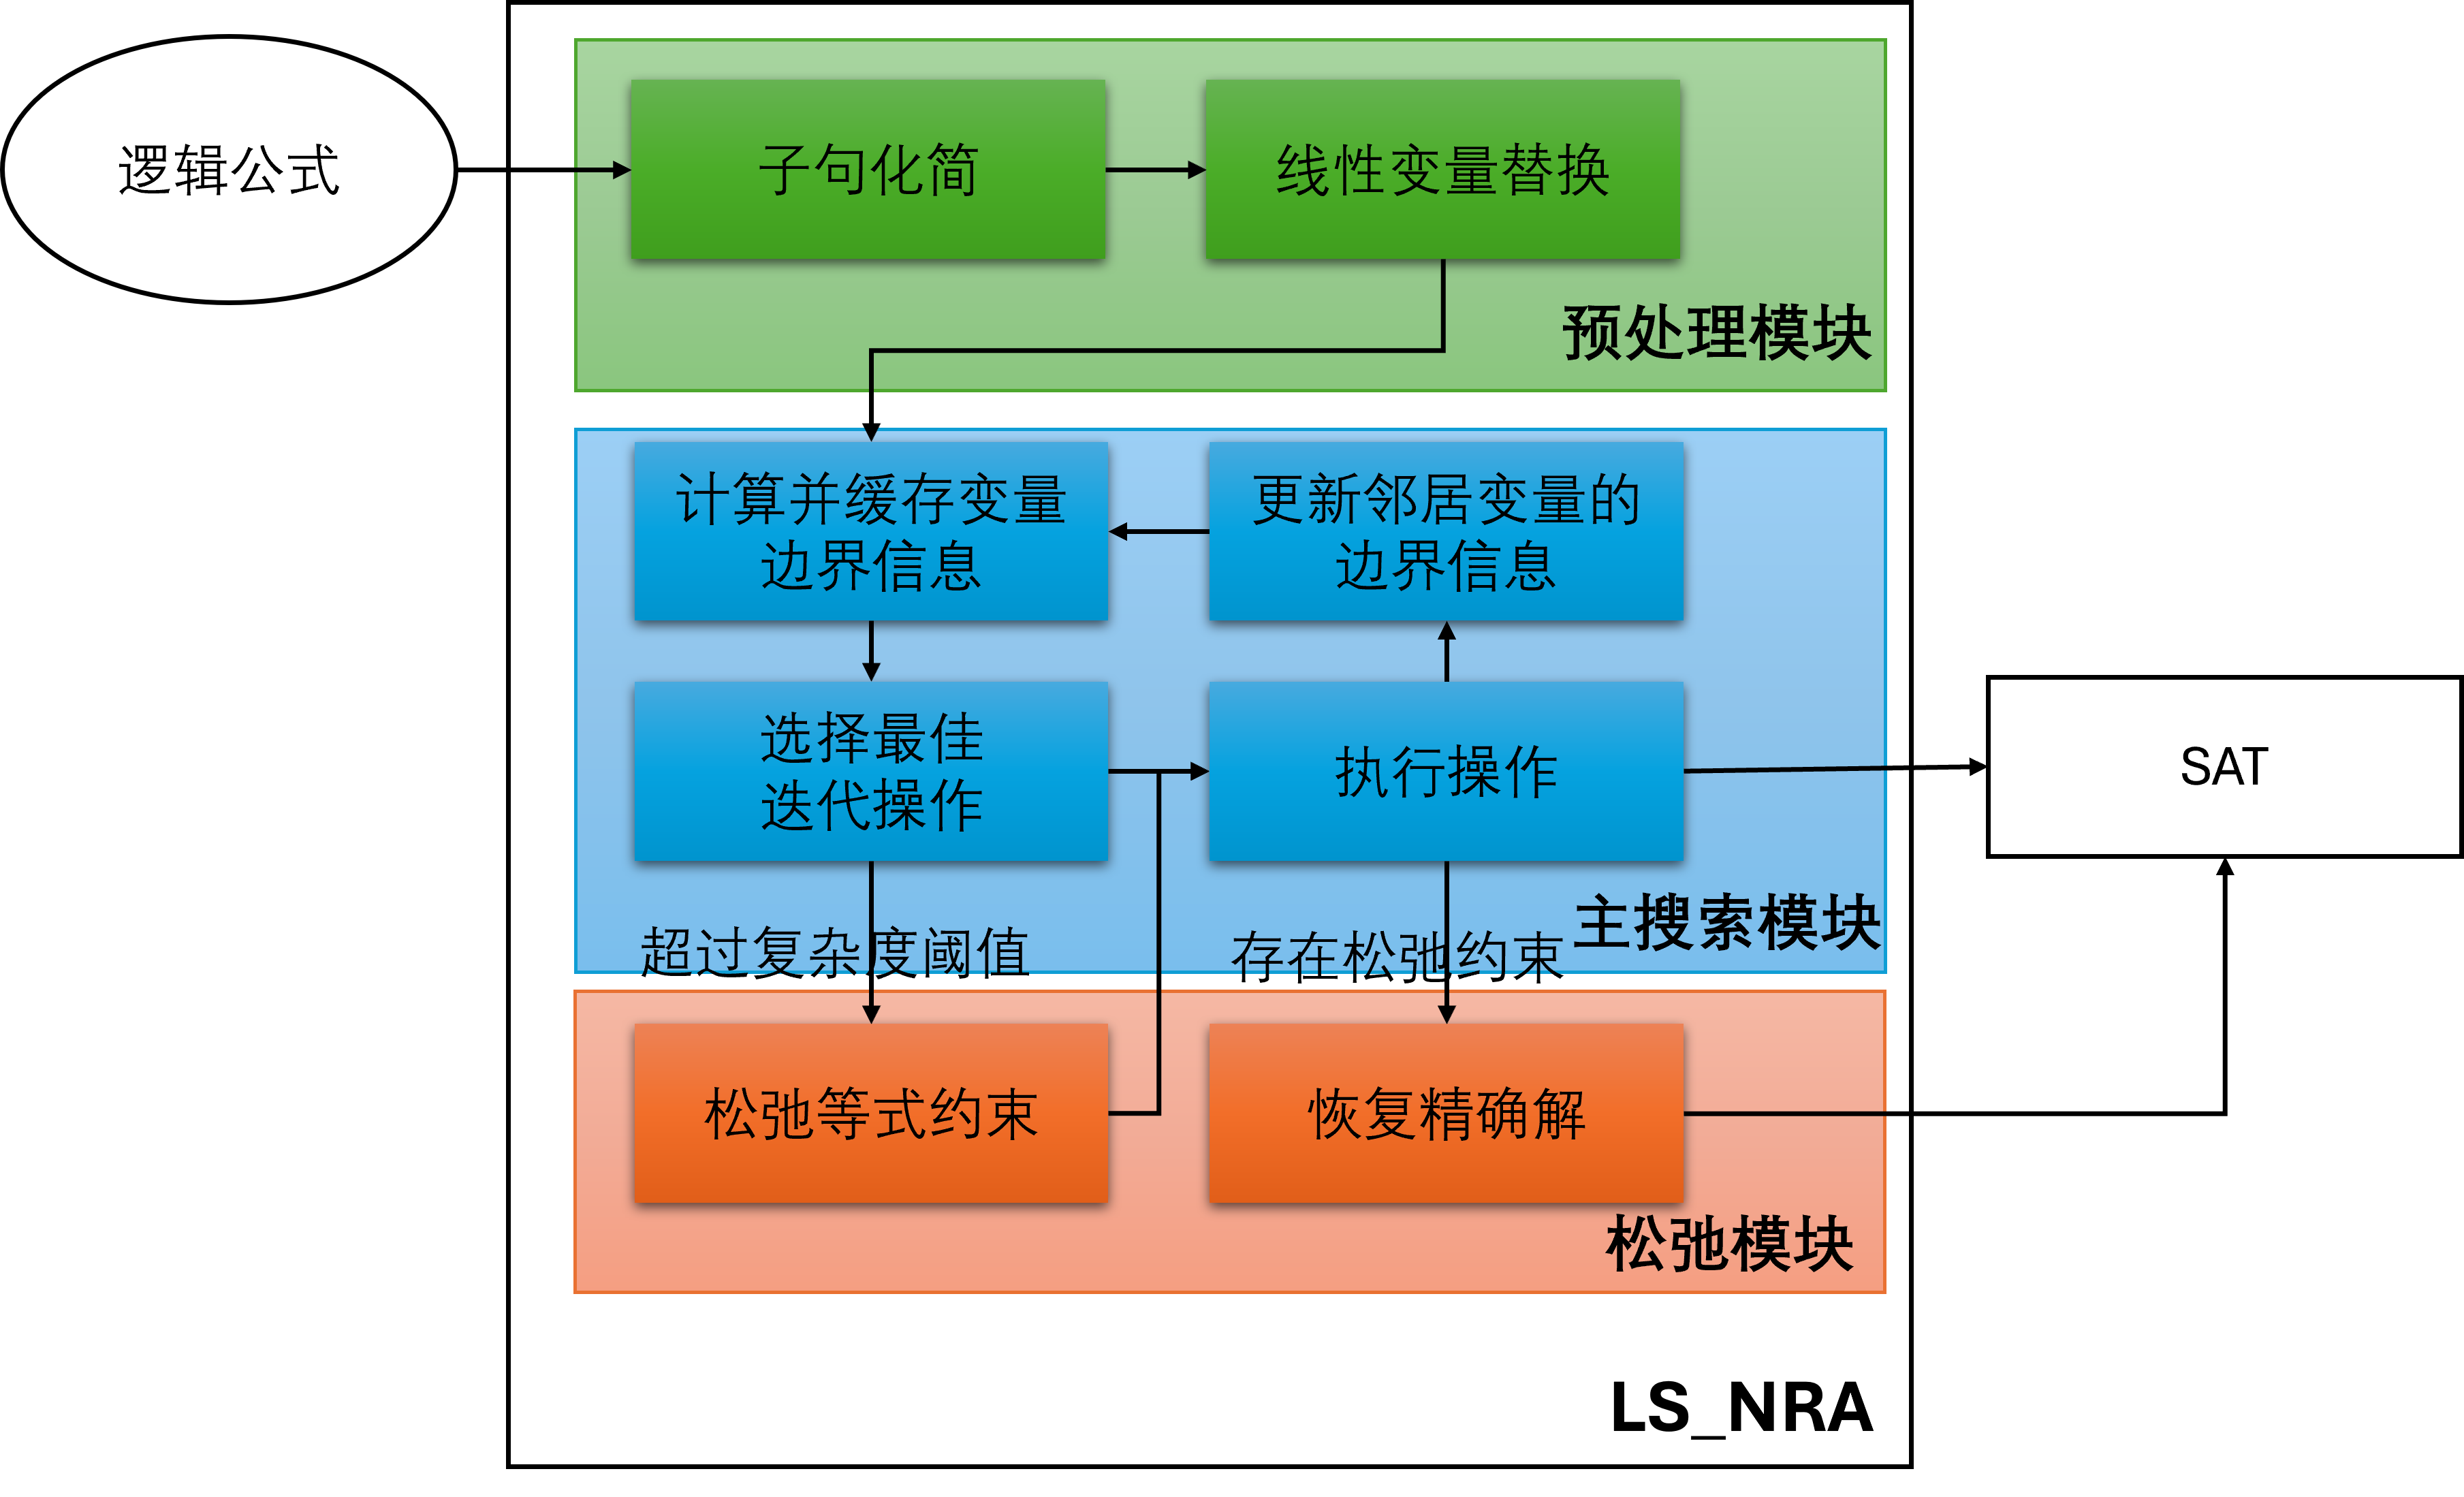
\includegraphics[width=0.9\columnwidth]{Img/structure.png}
    \label{fig:total}
\end{figure*}

\textbf{预处理阶段 (Preprocessing):} 预处理阶段主要负责化简主要的子句形式,以及简单的变量替换,为后续的主要搜索过程提供方便。
\begin{itemize}
    \item \textbf{子句化简 (Simplify):} 将同时出现的子句$p \le 0$和$p \ge 0$合并为$p = 0$。
    \item \textbf{变量替换 (Variable Substitution):} 在形如$c \cdot x + q = 0$的等式约束中,其中$c$是常数,$q$是次数最多为1的多项式并且最多包含2个变量,替换掉变量$x$。这里限制$q$的形式以降低变量替换的频率和计算复杂度。
\end{itemize}

\textbf{重启策略 (Restart):} 本工作设计了一个双层的重启策略,参数分别为$T_1$和$T_2$,值均为100。其中一次\textbf{小重启}在$T_1$次迭代没有改进后执行,随机选择未满足子句中的一个变量修改赋值。在$T_2$次小重启之后,一次\textbf{大重启}会重置所有变量的赋值。

\textbf{加权策略 (Weighting Scheme):} 本工作引入PAWS(pure additive weighting scheme)\cite{PAWS}作为加权策略。PAWS的基本思想是初始为每个子句设置权重为1,所有为满足的子句在局部最优时权重加1,当子句权重增加一定次数后一次性减少所有子句的权重。目前主流的SAT求解器比如EagleUP\cite{eagleup}和Sparrow2011\cite{sparrow}都采用了这种技术。

\textbf{线性方程的快速运算 (Shortcut for Linear Equations):} 本文的实根隔离是基于Z3现有的多项式操作库完成的,其原理是牛顿迭代法求解方程的根。但是当变量在多项式中以线性项出现时,可以通过斜率快速计算可行域,而非使用更通用的实根隔离函数。

\textbf{参数设置:} 本工作的可调参数设置如表\ref{tab:parameter}所示。

\begin{table*}[]
    \centering
    \bicaption{算法的可调参数设置} {Tunable parameters of the algorithm}
    \resizebox{0.7\linewidth}{!}{
        \begin{tabular}{c | c | c}
            符号 & 参数说明 & 预设值 \\\hline
            $sp$ & PAWS加权策略的概率 & 0.006\\\hline
            $T_1$ & 小重启执行所需的无提升迭代次数 & 100\\\hline
            $T_2$ & 大重启执行所需的小重启次数 & 100\\\hline
            $\epsilon_v$ & 等式松弛所需的复杂度阈值 & $10^{-4}$\\\hline
            $\epsilon_c$ & 等式松弛的程度 & $10^{-4}$\\\hline
        \end{tabular}
        }
\label{tab:parameter}
\end{table*}

\section{本章小结}
本章节主要讨论了LS\_NRA的实现细节,包括启发式移动和前瞻机制、预处理阶段、重启策略、线性方程的快速运算以及参数设置。具体来说,本工作给出了局部搜索算法中常见的停滞状态,然后给出了一种启发式候选赋值策略。接着,针对每个不同的环节给出了快速运算的策略,并且描绘了整体的结构示意图。